\chapter{Práctica 2: Preparación e Impresión de una Pieza}

\begin{center}
  \small\renewcommand{\arraystretch}{1.3}
  \begin{tabular}{l l l l}
    \textbf{Equipo:}      & Robo R2   &
    \textbf{Actividades:} & 3 \\
    \textbf{Software:}    & Cura for Robo &
    \textbf{Duración:}    & 2 horas \\
  \end{tabular}
\end{center}

\section{Introducción}

Para imprimir, el modelo 3D (\texttt{.stl}) debe convertirse en \texttt{.gcode} con un \textbf{laminador}. Cura for Robo es el software recomendado por el fabricante; ya trae perfiles preparados para la R2, de modo que el estudiante solo elige material y calidad. Después el archivo se envía a la impresora por USB o por el panel web.

\begin{objetivebox}
\begin{itemize}
    \item Preparar un modelo en Cura for Robo (material, calidad, orientación y soportes).
    \item Revisar el resultado en la vista de capas antes de imprimir.
    \item Imprimir desde la pantalla táctil y vigilar el progreso.
    \item Retirar la pieza sin dañarla ni dañar la lámina PEI.
\end{itemize}
\end{objetivebox}

\vspace{6pt}

\begin{materialbox}
\begin{itemize}
    \item Robo R2 calibrada y con filamento cargado (Práctica 1).
    \item Computador con Windows de 64 bits y Cura for Robo instalado.
    \item Archivo \texttt{.stl} de la pieza y memoria USB.
    \item Espátula, guantes y paño húmedo.
\end{itemize}
\end{materialbox}

\vspace{6pt}

\begin{infobox}[Temperaturas de referencia]
\begin{center}
\small
\begin{tabular}{l c c}
  \toprule
  \textbf{Material} & \textbf{Hotend} & \textbf{Cama (R2)} \\
  \midrule
  PLA & \grados{190}--\grados{210} & \grados{50} (hasta \grados{70}) \\
  ABS & \grados{230}--\grados{250} & \grados{80} (hasta \grados{100}) \\
  \bottomrule
\end{tabular}
\end{center}
Para el filamento Robo, \grados{190} es el valor óptimo de PLA y \grados{230} el de ABS.
\end{infobox}

\newpage
\section{Actividad 1: Laminar el modelo en Cura for Robo}

Cura for Robo requiere Windows de 64 bits y una tarjeta gráfica compatible con OpenGL~2. La primera vez que lo abra, el asistente pide elegir la impresora: seleccione \textbf{Robo R2} y pulse \ruta{Add Printer}.

\begin{enumerate}
    \item \textbf{Cargar el modelo:} icono \ruta{Open File} (arriba a la izquierda) y elija el \texttt{.stl}.
    \item \textbf{Elegir el material:} debe ser el mismo que está cargado en la impresora.
    \item \textbf{Elegir el perfil:} \emph{Low}, \emph{Medium}, \emph{High} o \emph{Ultra High Quality}. Mayor calidad significa capas más finas y más tiempo de impresión.
    \item \textbf{Ajustes rápidos:} densidad de relleno, adhesión a la cama (\emph{raft}) y estructuras de soporte para voladizos y puentes.
    \item \textbf{Orientar la pieza:} seleccione el modelo y use las herramientas \ruta{Move}, \ruta{Scale} (marque \emph{Uniform Scaling} para conservar proporciones), \ruta{Rotate} (\emph{Lay Flat} la apoya sobre una cara plana) y \ruta{Mirror}.
    \item \textbf{Revisar:} en la vista \emph{Layers} recorra las capas con el deslizador y confirme que la pieza se construye como espera. La vista \emph{X-Ray} marca en rojo huecos e intersecciones del modelo; si aparecen, corríjalos en el programa de diseño.
    \item \textbf{Exportar} el \texttt{.gcode} a la memoria USB.
\end{enumerate}

\begin{table}[H]
    \centering
    \caption{Ajustes de Cura que más influyen en el resultado.}
    \label{tab:cura}
    \small
    \begin{tabularx}{\linewidth}{l X}
        \toprule
        \textbf{Ajuste} & \textbf{Efecto} \\
        \midrule
        Altura de capa & Menor altura: más detalle y más tiempo. Mayor altura: menos detalle y más rápido. \\
        Grosor de paredes & Unas 3 veces el ancho de línea es un valor típico; más paredes dan una pieza más resistente. \\
        Relleno (infill) & Cerca de 20\,\% para piezas visuales; mayor para piezas mecánicas. \\
        Retracción & Reduce los hilos de plástico (stringing). Demasiada retracción puede dañar el filamento o tapar la boquilla. \\
        Velocidad & Los perfiles por defecto equilibran rapidez y vida útil; la primera capa se imprime más lenta para adherir mejor. \\
        \bottomrule
    \end{tabularx}
\end{table}

\newpage
\section{Actividad 2: Imprimir y vigilar}

\subsection*{Iniciar desde la memoria interna}

\begin{enumerate}
    \item En la pantalla de inicio seleccione \ruta{Files} y elija el archivo.
    \item Pulse \ruta{Start} y espere unos segundos mientras la impresora se prepara.
\end{enumerate}

\subsection*{Iniciar desde una memoria USB}

\begin{enumerate}
    \item Inserte la USB en la ranura frontal.
    \item \ruta{Files}\flecha elija el archivo.
    \item Decida si lo copia a la impresora o lo imprime directamente desde la USB.
    \item Pulse \ruta{Start}.
\end{enumerate}

\subsection*{Vigilar la impresión}

La pestaña \ruta{Printer} muestra el nombre del archivo, el porcentaje de avance, el tiempo y las temperaturas. Desde ahí puede pulsar \ruta{Pause} o \ruta{Cancel}, o tocar la temperatura del extrusor para modificarla. También puede seguir el estado desde la app o el panel web (Práctica 3).

\begin{figure}[H]
    \centering
    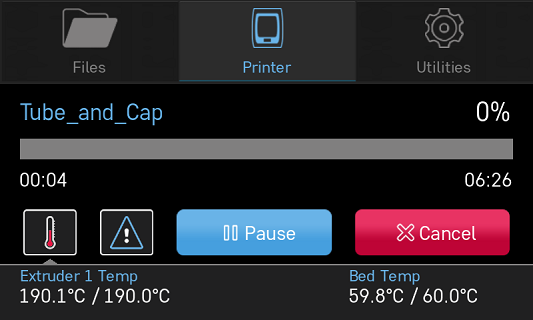
\includegraphics[width=0.55\linewidth]{r2_impresion.png}
    \caption{Pestaña \emph{Printer} durante una impresión: progreso, temperaturas y botones Pause/Cancel.}
    \label{fig:impresion}
\end{figure}

\begin{warningbox}
No deje la impresora sin supervisión y vigile la \textbf{primera capa}: es donde se detectan los problemas de adhesión. Si la boquilla arrastra o el plástico no se pega, cancele y repita la calibración del Z-Offset.
\end{warningbox}

\section{Actividad 3: Retirar la pieza y evaluar}

\begin{enumerate}
    \item Espere a que la pieza y la cama se enfríen.
    \item Retire la cama con las dos manos y colóquela sobre una superficie plana.
    \item Con la espátula, levante la pieza por los bordes y avance poco a poco por debajo. \textbf{No tire de la pieza hacia arriba} desde el centro: puede romperse.
    \item Limpie la lámina PEI con un paño húmedo antes de la siguiente impresión.
    \item Al volver a colocar la cama, verifique que los imanes calcen y que el cable de alimentación de la cama esté conectado: si no está bien asentada, la impresión falla.
\end{enumerate}

\begin{infobox}[Si la pieza ya no se pega]
La lámina PEI dura aproximadamente de 4 a 6 meses. Si las piezas dejan de adherirse, líjela suavemente con lija de grano 2000 y límpiela con un paño húmedo. Luego repita la calibración del Z-Offset.
\end{infobox}

\section{Entregables}

\begin{entregabox}
\begin{itemize}
    \item Captura de Cura for Robo con el modelo, material y perfil elegidos, y de la vista de capas.
    \item Fotografía de la pieza impresa y tiempo total de impresión.
    \item Breve análisis: ¿cómo salió la primera capa? ¿Qué ajuste cambiaría y por qué?
\end{itemize}
\end{entregabox}
